\section{Simulation Results}\label{sec:simulations}

We now explore simulation results from the model considering a wide range of choices for the speculator's risk constraint. Unless otherwise noted, the simulations use the following parameter set with a simplified constant demand assumption ($\mathcal{D}=100$) and a t-distribution with df=3 to simulate Ether log returns. This carries over the simplified model from Section~\ref{sec:stable_v_unstable}, although other choices are also amenable to simulation. Cryptocurrency returns are well known for having very heavy tails. This choice gives us these heavy tails with finite variance. Note, however, that this doesn't capture path dependence of Ether returns. We instead assume Ether returns in each period are independent. We run simulations on 10k paths of 1000 steps (days) each. This is enough time to look at short-term failures and dynamics over time. The simulation code is available with full details at \url{https://github.com/aklamun/Stablecoin_Deleveraging}.

\begin{center}
	\begin{tabular}{c|l|l}
		\textbf{Parameter}	&	\textbf{Value}	& \textbf{Rationale} \\
		\hline
		$n_0$		&	$400$ 	&	4x initial collateralization $>$ typical Dai level \\
		$r_0$		&	$1.00583$	& Historical daily Ether mult. return 2017-2018 \\
		$\mu_0$		&	$0.00162$	& Historical daily Ether log return 2017-2018 \\
		$\sigma_0$	&	$0.027925$	& Historical daily Ether volatility 2017-2018 \\
		$\gamma=\delta$	&	$0.1$	& $\sim$ Recommended value \cite{longerstaey1996} \\
		%$\delta$	&	$0.1$	& $\sim$ Recommended value \cite{longerstaey1996} \\
		$\beta$		&	$1.5$	& Threshold used in MakerDAO's Dai \\
		$\alpha$	&	$\sim 1.28$	& Value assuming normal distr. + $a=0.1$ \\
		$b$		&	$1$	& Consistent with VaR constraint \\
		%$\sigma_{-}$		&	$0$	& Consistent with VaR constraint
	\end{tabular}
\end{center}


Note that our simulations study daily movements. We choose this time step to examine these systems under reasonable computational requirements. More realistic simulations might study intraday movements. One plausible scenario of a Dai freeze is if the price feed moves too far too fast instraday, so that speculators don't have enough time to react before liquidations are triggered and keepers (who perform actual liquidations) are unable to handle the avalanche of liquidations. As the price feed in Dai faces an hourly delay in the price feed, hourly time steps are a natural choice for follow-up simulations. This said, daily time steps can actually be reasonable due to a behavioral trend in Dai data: most Dai speculators realistically don't track their positions with very high frequency as supported by overall high liquidation rates.





%%%%%%%%%%%%%%%%%%%%%%%%%%%%%%%%%%%%%%%%%%%%%%%%%%%%%%%%%%%%%%%%
\subsection{Speculator behavior affects volatility}
We compare DStablecoin performance under the following speculator behaviors encoded in the risk constraint.
\begin{center}
	\begin{tabular}{c|l}
		\textbf{Name}	&	\textbf{Speculator risk constraint} \\
		\hline
		VaRN.1	&	 VaR using $a=0.1$ + normality assumption \\
		VaRN.01	&	VaR using $a=0.01$ + normality assumption \\
		VaRM.1	&	VaR using $a=0.1$ + heavy-tailed assumption \\
		VaRM.01	&	VaR using $a=0.01$ + heavy-tailed assumption \\
		AC1		&	Anti-cyclic constraint, $b=-0.5$, $\alpha=0.01$ \\
		AC2		&	Anti-cyclic constraint, $b=-0.5$, $\alpha=0.02$ \\
		RN		&	Risk neutral, only faces liquidation constraint
	\end{tabular}
\end{center}

Figure~\ref{fig:vol_risk_mgmt} compares the effects on volatility of these behavioral constraints under various Ether return distributions. These figures are heatmaps/2D histograms similar to that in Figure~\ref{fig:hist_vol_learning_rate}. The results suggest that DStablecoins face significant tail volatility (on the order of Ether volatility) even under comparatively `nice' assumptions on Ether return distributions, such as with significant upward drift (Figure~\ref{fig:hist_vol_risk_mgmt_drift_nz}) and a normal distribution (Figure~\ref{fig:hist_vol_risk_mgmt_normal}). Figure~\ref{fig:simulation_msd} depicts relative (\% difference) mean-squared difference of simulated volatility for the different risk management methods vs. a risk neutral speculator. The mean-squared difference is large, suggesting that the speculator's risk management method has a large effect on volatility.

The results suggest how speculator behavior can affect DStablecoin volatility within the model. Stricter cyclic risk management (e.g., VaR) on the part of the (single) speculator can lead to increased DStablecoin volatility without improving the safety of the system. Whether countercyclic (setting constraint to increase leverage during downturns) or cyclic (setting constraint to decrease leverage during downturns), the resulting DStablecoin volatility is connected with how narrow the feasible region for the constraint becomes. A risk neutral speculator, which has the widest feasible region for the constraint, leads to the lowest volatility. Stricter risk management serves to reduce the feasible region. Note that these results may be different if there are multiple types of speculators, for instance some that are cyclic and others that are countercyclic.

Figure~\ref{fig:hist_vol_learning_rate} further suggests that a higher speculator memory parameter (lower memory) tends to increase volatility in typical cases. This makes sense as high memory parameters can lead to noise chasing on the part of the speculator. Note that keeping the speculator's expected Ether returns and variance constant is equivalent to setting a static risk constraint.

\begin{figure}
	\centering
	\begin{subfigure}[b]{0.49\textwidth}
		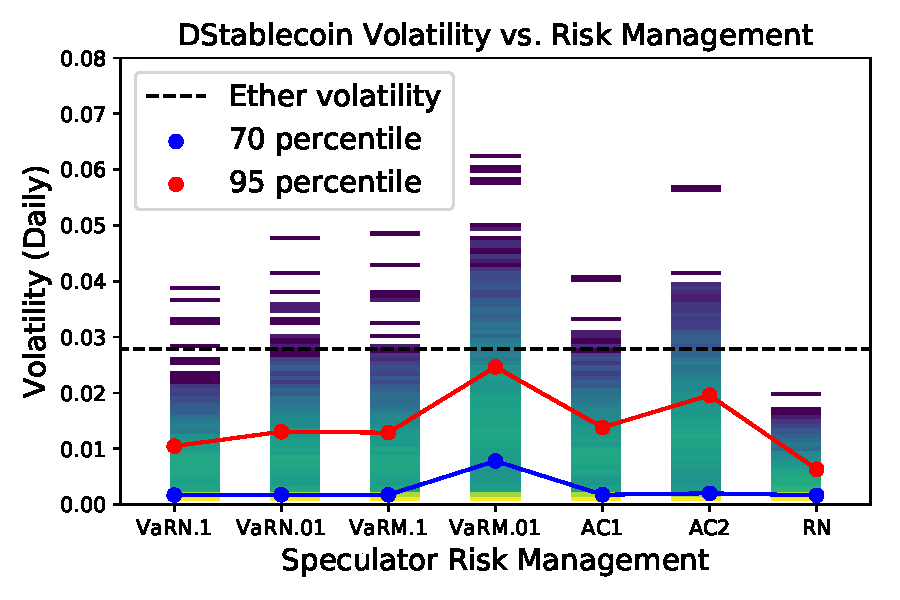
\includegraphics[width=\textwidth]{figures/hist_vol_risk_mgmt_tdist}
		\caption{Ether returns$\sim\text{t-distr}(\text{df}=3,\mu=0)$}\label{fig:hist_vol_risk_mgmt_tdist}
	\end{subfigure}
	\begin{subfigure}[b]{0.49\textwidth}
		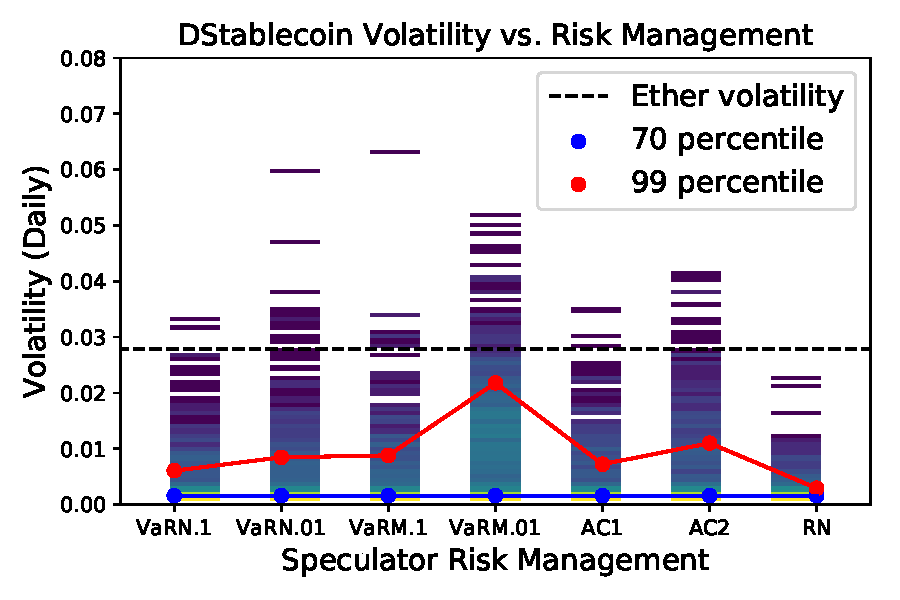
\includegraphics[width=\textwidth]{figures/hist_vol_risk_mgmt_drift_nz}
		\caption{Ether returns$\sim\text{t-distr}(\text{df}=3,\mu=r_0)$}\label{fig:hist_vol_risk_mgmt_drift_nz}
	\end{subfigure}
	\begin{subfigure}[b]{0.49\textwidth}
		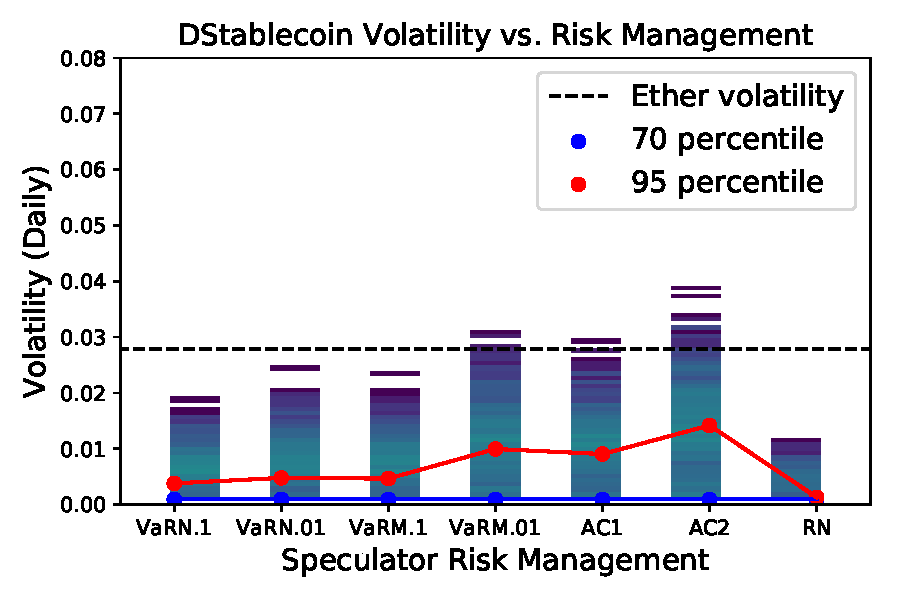
\includegraphics[width=\textwidth]{figures/hist_vol_risk_mgmt_normal}
		\caption{Ether returns$\sim\text{normal}(\mu=0)$}\label{fig:hist_vol_risk_mgmt_normal}
	\end{subfigure}
	\caption{Heatmaps of DStablecoin volatility for different speculator risk management behaviors.}\label{fig:vol_risk_mgmt}
\end{figure}






%%%%%%%%%%%%%%%%%%%%%%%%%%%%%%%%%%%%%%%%%%%%%%%%%%%%%%%%%%%%%%%%
\subsection{Stable asset failure is dominated by collateral asset returns}
We define the DStablecoin's \textbf{failure (or stopping) time} to be either (1) when the speculator's liquidation constraint is unachievable or (2) when the DStablecoin price remains below \$0.5 USD. In these cases, a global settlement would be reasonable, leaving DStablecoin holders with Ether holdings with high volatility in subsequent periods.

Figure~\ref{fig:stopping_risk_mgmt} compares the effects on failure time of these behavioral risk constraints. The stopping time distributions appear comparable across a wide range of selections for the speculator's risk constraint. They are additionally comparable across the memory parameters studied above. Figure~\ref{fig:simulation_msd} depicts relative mean-squared difference of simulated stopping times for the different risk management methods vs. a risk neutral speculator. In calculating the mean-squared difference, we only include cases in which the failure is realized within the simulation. The mean-squared difference is small (1-2 orders of magnitudes smaller than for volatility), providing additional evidence that the stopping time is largely independent of the speculator's risk management. In particular, a large proportion of failure events would not have been prevented by different speculator risk management within the model.

DStablecoin failure probabilities appear to be dominated by Ether returns as opposed to speculator behavior. The results suggest that DStablecoins may not be long-term stable, even under comparatively `nice' assumptions for Ether return distributions. To avoid failure, they would essentially rely on more speculator capital entering the system during downturns.


\begin{figure}
	\centering
	\begin{subfigure}[b]{0.49\textwidth}
		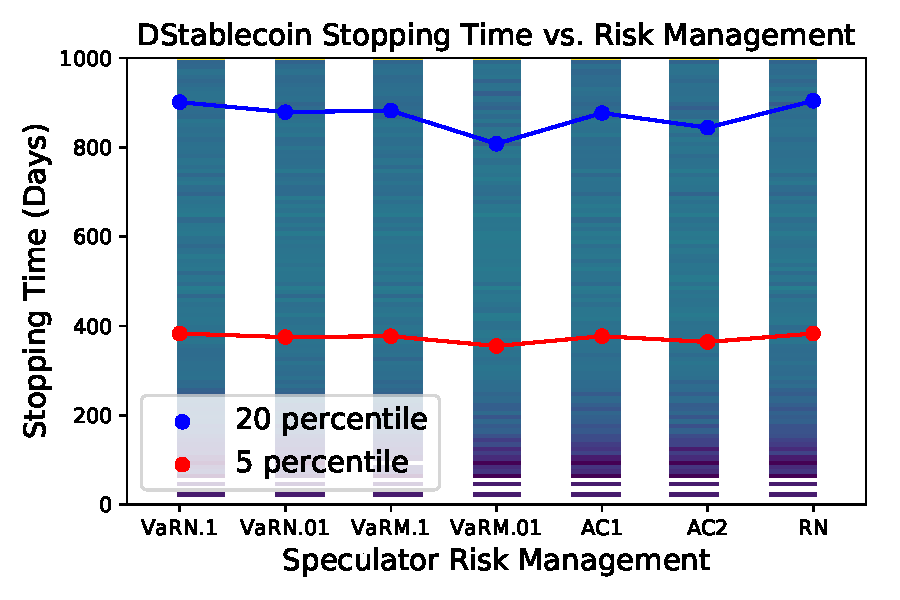
\includegraphics[width=\textwidth]{figures/hist_stopping_risk_mgmt_tdist}
		\caption{Ether returns$\sim\text{t-distr}(\text{df}=3,\mu=0)$}\label{fig:hist_stopping_risk_mgmt_tdist}
	\end{subfigure}
	\begin{subfigure}[b]{0.49\textwidth}
		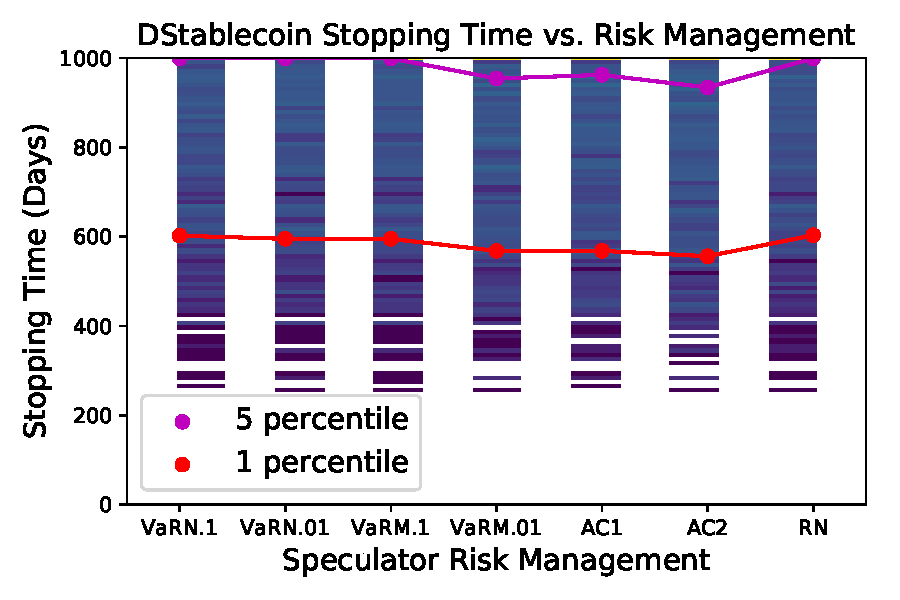
\includegraphics[width=\textwidth]{figures/hist_stopping_risk_mgmt_normal}
		\caption{Ether returns$\sim\text{normal}(\mu=0)$}\label{fig:hist_stopping_risk_mgmt_normal}
	\end{subfigure}
	\caption{Heatmaps of DStablecoin failure times for different speculator risk management behaviors.}\label{fig:stopping_risk_mgmt}
\end{figure}



\begin{figure}
	\centering
	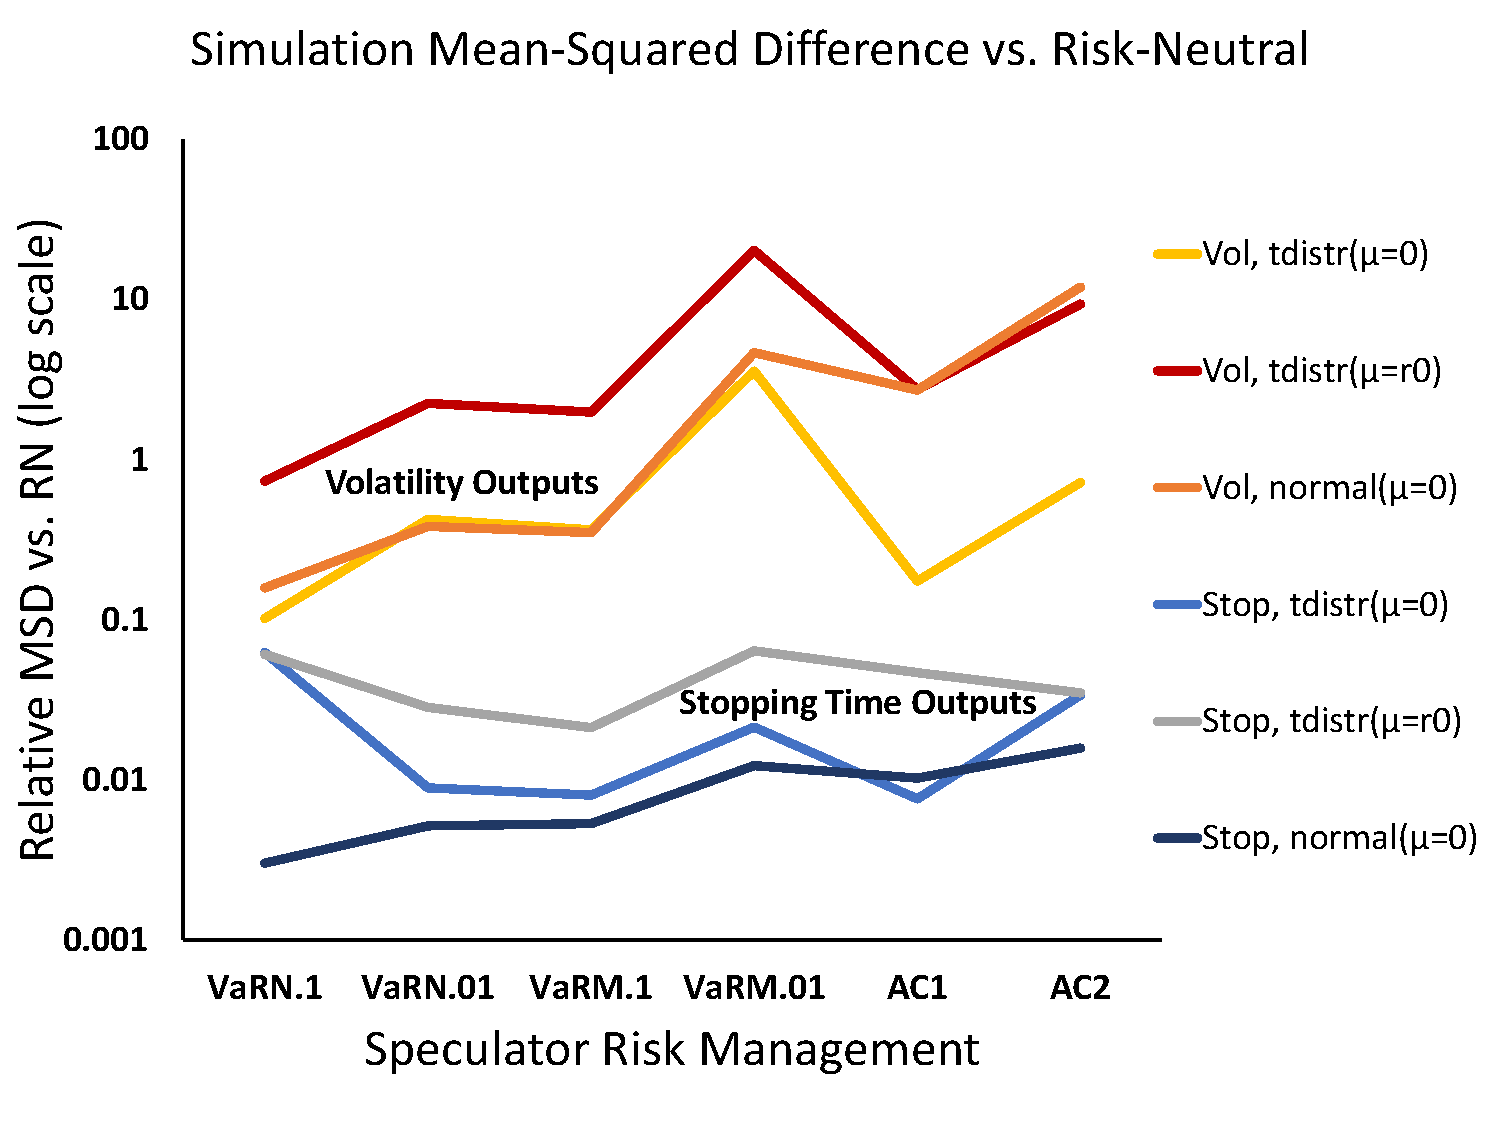
\includegraphics[width=0.7\textwidth]{figures/simulation_msd_figure_2}
	\caption{Relative mean-squared difference (MSD) of simulated volatility and stopping time for given speculator strategy vs. risk neutral strategy. Different lines represent different output (volatility or stopping time) and different return distribution assumptions for the simulations.}\label{fig:simulation_msd}
\end{figure}






